\chapter{Background}
This chapter serves as a fundamental cornerstone in the overall structure of this thesis, as it is designed to provide a comprehensive and in-depth exploration of several key areas of study that are crucial to the understanding of the research presented in the subsequent chapters. Through a detailed exposition, this chapter illuminates the foundational principles and contextual factors that underlie the entire thesis.

The first component of this chapter is dedicated to elucidating the intricate domain of information retrieval, a field that is pivotal in the context of this research. Information retrieval is the process of obtaining relevant information from vast collections of data, and it encompasses various techniques and methodologies aimed at achieving this objective. By delving into this subject matter, the reader is equipped with the essential knowledge to appreciate the challenges and complexities of the thesis's research focus.

Large language models, which are a central focus of this work, are introduced and discussed in this chapter. These models represent a breakthrough in natural language processing and artificial intelligence, capable of comprehending and generating human-like text at an unprecedented scale. Their significance lies in their potential to enhance information retrieval systems, an integral aspect of this research. The chapter expounds on the architecture, capabilities, and potential applications of these models, laying the groundwork for the subsequent exploration of their role in the thesis.

The evaluation of retrieval pipelines, a critical research component, is also thoroughly examined in this chapter. It elucidates the methodologies and metrics used to assess the performance and effectiveness of information retrieval systems. An understanding of evaluation techniques is vital for comprehending the empirical aspects of the research and how improvements in retrieval pipelines are quantified and validated.

Moreover, this chapter introduces the concept of query variations, a pivotal notion that forms the bedrock of subsequent research endeavours. Query variations involve the diversification and adaptation of search queries to enhance the quality and relevance of retrieved information. The chapter explores the rationale behind this concept, its significance, and its potential impact on information retrieval systems, setting the stage for the research that follows.

\section{Information Retrieval}
Information Retrieval (IR) is a multifaceted process that plays a pivotal role in the digital age, enabling users to access specific, pertinent information from vast and often overwhelming data collections, including text documents, websites, or other data sources. IR systems employ a diverse array of techniques and algorithms to meticulously analyse, index, and make sense of these extensive datasets, thereby enabling efficient and accurate search processes. Commonly encountered forms of these datasets include search engine indexes, document repositories, or databases, and they are meticulously structured to facilitate rapid retrieval and ranking of information.

When a user initiates a search by entering a query into an IR system, a complex sequence of operations unfolds. The IR system, powered by sophisticated algorithms, scrutinises the indexed data to pinpoint documents, web pages, or other data sources most relevant to the user's query. The system then assembles these search results into a coherent and ranked list, with the most pertinent information at the top. This step is crucial in ensuring users find the information they seek efficiently, minimising the need for manual sifting through extensive data collection.

To illustrate the systematic flow of an information retrieval system, \fig{fig:pipelines} depicts the step-by-step process through which a user's query is transformed into relevant search results. Each component in the process, such as query processing, document retrieval, ranking, and result presentation, is instrumental in delivering a seamless and user-friendly information retrieval experience.

\subsection{Large Language Models}
\begin{figure}
    \centering
    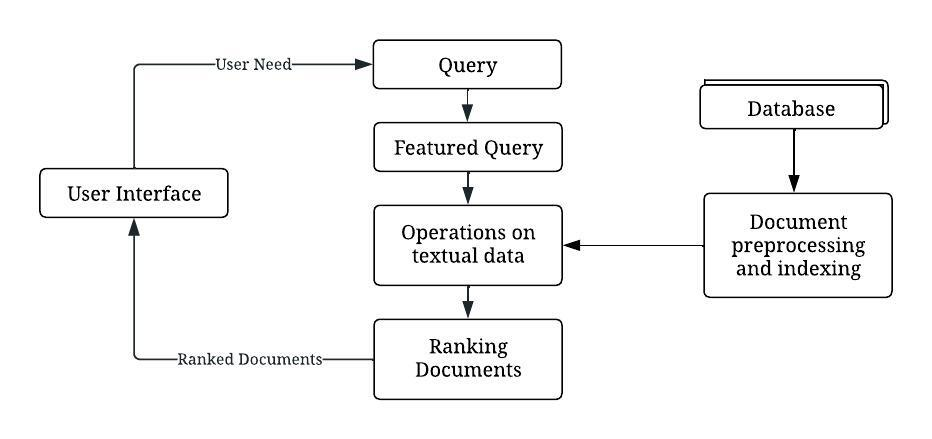
\includegraphics[width=\textwidth]{2Background/Background/IR.jpeg}
    \caption{Flowchart illustrating the information retrieval system process.}
    \label{fig:pipelines}
\end{figure}

Large Language Models (LLMs), often called state-of-the-art language models in Natural Language Processing (NLP), represent a remarkable advancement in machine learning technology. These models are designed to handle vast amounts of text data, allowing them to generate natural language text, answer questions, or make predictions. LLMs like GPT-3 and BERT have gained significant attention for their ability to comprehend and generate human-like text \cite{penha2022}.

LLMs find applications across a wide array of real-world scenarios. They power chatbots, which can engage in human-like conversations, making them invaluable for customer support and virtual assistants. They are integral in language translation services, breaking down language barriers and enabling seamless communication between individuals who speak different languages. Moreover, LLMs are the foundation for voice assistants, such as Siri or Alexa, enhancing their natural language understanding and response capabilities \cite{gpt}.

In addition to these applications, LLMs have unlocked new possibilities in content generation, language modelling, and text summarisation. They can craft coherent articles, stories, or reports, and they can serve as a foundation for more advanced language models. They can also distil lengthy documents into concise summaries, immensely valuable for tasks like content curation and automated news aggregation. Their versatility in understanding and generating text has made them a cornerstone of modern NLP research and applications.

Now, turning our attention to the domain of Information Retrieval (IR), retrieval pipelines play a pivotal role in efficiently searching and retrieving relevant information from extensive data collections, be it a document database or a search engine index. These pipelines encompass a series of well-defined processing steps to streamline the retrieval process:

\begin{itemize}
    \item Query Processing: This initial step involves processing user queries. During query processing, the system identifies relevant terms, expands the query with synonyms, and applies other query optimisation techniques to enhance the accuracy of the retrieval process.
    \item Document Indexing: In this step, the documents contained within the collection are indexed. Document indexing involves the transformation of documents into a more manageable format, often through token embedding techniques. This transformed data structure facilitates faster and more efficient searching.
    \item Ranking: Following document indexing, documents are ranked based on their relevance to the user's query. Various models and algorithms are applied to assign scores to documents, allowing for the sorting of documents by their perceived relevance.
    \item Presentation: The final stage of the retrieval pipeline involves presenting the search results to the user in a user-friendly format. This could be a list of documents with summaries, snippets, or other relevant metadata, making it easier for users to find and access the information they seek \cite{chen, zendel}.
\end{itemize}

It's important to note that retrieval pipelines can be further customised to cater to specific needs. Additional steps might include filtering or classifying search results based on domain-specific criteria or leveraging machine learning techniques to improve relevance comparisons. These advanced steps are particularly relevant in scenarios where precise and contextually relevant results are essential, such as in medical information retrieval \cite{lu}.
\section{Natural Language Processing}
\subsection{Ranking}
Ranking is a pivotal component within information retrieval systems, central to organising a collection of textual documents or search results based on their relevance to a given query or topic. The ranking process in these algorithms involves utilising multiple features to assign numerical scores to individual documents. These scores subsequently serve as the basis for arranging the documents in descending order, ensuring that the most pertinent ones appear at the forefront of the list \cite{wu}.

The significance of ranking transcends many applications, impacting the functionality of diverse systems, including search engines, chatbots, and question-answering platforms \cite{nlp}. To comprehend the ranking process, it is essential to consider several key aspects:

\begin{itemize}
    \item Feature Assessment: Ranking algorithms employ sophisticated techniques to assess and quantify the relevance of documents. These techniques encompass many factors, including keyword matching, semantic analysis, user behaviour patterns, and contextual cues.
    \item User-Centric Adaptation: Ranking algorithms operate dynamically, allowing information retrieval systems to adapt to evolving user queries and content. This adaptability ensures that users receive increasingly accurate and context-aware results.
    \item Enhanced User Experience: The impact of ranking extends to user experience and system performance. By prioritising the presentation of the most relevant content, ranking algorithms enhance user satisfaction and the overall efficiency of information retrieval processes.
    \item Ongoing Advancements: The ranking field continually evolves, with the integration of advanced machine learning and natural language processing methods contributing to the refinement of information retrieval systems. These advancements enhance their effectiveness and applicability across a broad spectrum of domains \cite{nlp}.
\end{itemize}

\subsection{Rank Fusion}
In information retrieval, rank fusion is a valuable technique that amalgamates ranked document lists generated by multiple retrieval methods or models. The primary objective is to enhance the retrieval process's overall efficacy by integrating outcomes from various sources.

The fundamental concept underlying rank fusion revolves around assigning scores or weights to individual documents within the ranked lists acquired from diverse retrieval methods. These set values are subsequently employed in constructing a novel merged list where documents are arranged based on their rankings. A commonly utilised approach for rank fusion is Reciprocal Rank Fusion (RRF) \cite{rankfusion}.

RRF is a technique used in information retrieval to combine the rankings generated by multiple retrieval methods or queries. It's advantageous when you have different sources of ranking scores, such as various retrieval models or query variations, and you want to aggregate them to improve overall retrieval performance. The core idea behind RRF is to assign a reciprocal rank score to each document in the individual rankings \cite{rankfusion}. Reciprocal rank is a measure that gives higher scores to documents that appear higher in the rankings. Then, these reciprocal rank scores from different rankings are summed up for each document, and the documents are re-ranked based on this aggregated score.

Rank fusion is advantageous when distinct retrieval techniques possess complementary strengths and weaknesses. Combining their findings makes it feasible to bolster overall performance in retrieving relevant documents while potentially enhancing quality standards. Nevertheless, meticulous design and evaluation of rank fusion methodologies remain crucial to effectively capture each source's advantages and generate meaningful merged rankings accordingly.

\subsection{Training}
Training denotes the process of instructing a machine learning model to perform specific linguistic tasks with a high degree of accuracy. These tasks encompass a wide range, including but not limited to text classification, sentiment analysis, and machine translation, and are pivotal to the broader field of NLP \cite{bert}. During the training, a substantial corpus of text data is input into the model, paired with corresponding target labels that convey the desired output for each input example. Through iterative exposure to this labelled data, the model endeavours to discern intricate relationships and patterns that underlie the language-based tasks at hand \cite{nlp}.

The training phase is characterised by recurrent data processing, often called epochs. Throughout these iterations, the model's internal parameters are fine-tuned to progressively enhance its capacity to make accurate predictions and generate meaningful linguistic representations. This fine-tuning is facilitated by optimisation techniques that adjust the model's parameters to optimise its overall performance. The ultimate objective of the training process is to cultivate models that exhibit high accuracy in their predictions and operate with computational efficiency. These well-trained models are then deployed across various NLP applications, where they can efficiently process natural language text, offering valuable insights and enabling a myriad of language-related tasks to be automated and executed effectively.

\section{Effectiveness Evaluation}
The effectiveness of Large Language Models (LLMs) is a critical aspect of their assessment, and it is typically evaluated through a combination of offline and online methods, as well as user studies. These evaluations help gauge how well LLMs perform on various Natural Language Processing (NLP) tasks, ultimately contributing to their refinement and development.

\subsection{Offline Evaluation}
Offline evaluation is a commonly used method for assessing LLM effectiveness. It involves conducting evaluations on benchmark datasets with well-defined NLP tasks. These tasks can range from language translation to sentiment analysis and text classification. One widely used benchmark is the BM25 benchmark, along with various other similar datasets tailored to specific NLP tasks. The results of these offline evaluations provide a means to compare different LLMs and identify areas that may require improvement \cite{penha2022}.

\subsection{Online Evaluation}
Online evaluation is another crucial technique used to assess the effectiveness of LLMs, particularly in real-world, live applications. Instead of using pre-existing datasets, online evaluation involves deploying LLM systems in actual settings and measuring their performance and impact on user outcomes. This approach allows for observing how users interact with the system during live usage, providing insights into real-world effectiveness and efficiency improvements. This contrasts offline evaluations, which are based on historical data sets.

\subsection{User Studies}
In addition to data-centric evaluations, the effectiveness of LLMs can also be evaluated through user studies. User studies typically involve soliciting user feedback and collecting data on user satisfaction and experience. This feedback can be gathered through surveys or usability testing, where users are asked to perform specific tasks or interact with the LLM system. These studies provide valuable insights into how LLMs perform regarding user engagement, usability, and overall satisfaction.

\subsection{Metrics}
To quantify the effectiveness of LLMs, various metrics are used, each shedding light on different aspects of system performance. The choice of metric depends on the specific evaluation context and the goals of the assessment. One primary evaluation metric often employed in information retrieval is nDCG (Normalised Discounted Cumulative Gain).

nDCG (Normalised Discounted Cumulative Gain): nDCG is a widely recognised metric in information retrieval, particularly relevant when the order of search results is crucial. It assesses the quality of ranked lists by considering the relevance of documents and their positions within the list. It calculates cumulative gain attributed to relevant documents while appropriately discounting the importance of items lower down the ranking. Normalisation ensures that nDCG values fall within the range of 0 to 1, making it suitable for comparisons across different retrieval tasks and datasets. nDCG is sensitive to subtle distinctions in ranking order, which can significantly impact user satisfaction.
In addition to nDCG, there are several other standard metrics used in information retrieval evaluation, including:

\begin{itemize}
    \item Accuracy: Measures the percentage of correctly classified instances from all instances in the dataset.
    \item Precision: Measures the proportion of true positives (correctly classified documents) versus all documents classified as positive.
    \item Recall: Measures the proportion of true positives out of all positive documents.
    \item fMeasure: A harmonic mean of recall and precision, commonly used in imbalanced datasets to emphasise recall over precision.
    \item MAP (Mean Average Precision): Unlike the above measures, MAP accounts for all relevant document rankings by calculating the mean of precision scores across all queries. This provides a more comprehensive view of system performance \cite{sokolova}.
\end{itemize}

These metrics collectively contribute to a nuanced understanding of the retrieval process and the outcomes of LLMs in various NLP tasks and information retrieval scenarios.
\section{Query Variations}
\note{add diagram}
Query variation is a fundamental concept in information retrieval, encompassing a wide array of expressions and formulations that users employ when seeking specific information or conducting online searches \cite{zendel}. These variations can take shape in numerous ways, including alterations in word order, sentence structure, and shifts in phrasing. To illustrate, let's delve into the realm of baking and consider two queries: "How to bake a cake from scratch?" and "Homemade cake recipe?" Although these two queries exhibit nuanced differences, they essentially convey the same information need, showcasing the diverse ways in which users can articulate their search intents.

Query variations span a broad spectrum, encompassing distinct categories, each with its unique characteristics and challenges. Some common categories of query variations include specialization, aspect change, misspelling, natural language transformation, and paraphrasing \cite{penha2022}. Specialization involves refining a general query into a more specific one; aspect change entails altering the focus of the query while retaining the core intent; misspelling can introduce errors or typos; natural language transformation might involve changing from a question to a statement and paraphrasing entails expressing the same information need in different words.

Addressing query variation is of paramount importance in the field of information retrieval because it has a profound impact on the performance and effectiveness of search systems. Recognizing and accommodating the diverse ways users express their information needs is pivotal for enhancing the capacity of information retrieval (IR) systems to retrieve relevant documents. Several techniques are employed to manage query variation effectively in IR systems, including query suggestion, reformulation, and expansion.

Query Expansion: Query expansion is a technique used to broaden the scope of the original query. This is achieved by adding synonyms, related terms, or additional keywords to the initial query. The goal is to retrieve a more comprehensive set of relevant documents and improve the recall of the search results.

Query Reformulation: Query reformulation involves transforming the initial query into a new one that better aligns with the user's information needs. This can include changing the wording, structure, or focus of the query to increase its precision and relevance to the user.

By implementing these techniques and considering the multifaceted nature of query variations, IR systems can provide users with an enhanced and more tailored search experience. This not only improves the quality of search results but also ensures that users can find the information they need, even if their queries vary in expression and formulation.